\documentclass{standalone}
\usepackage{tikz}

\begin{document}
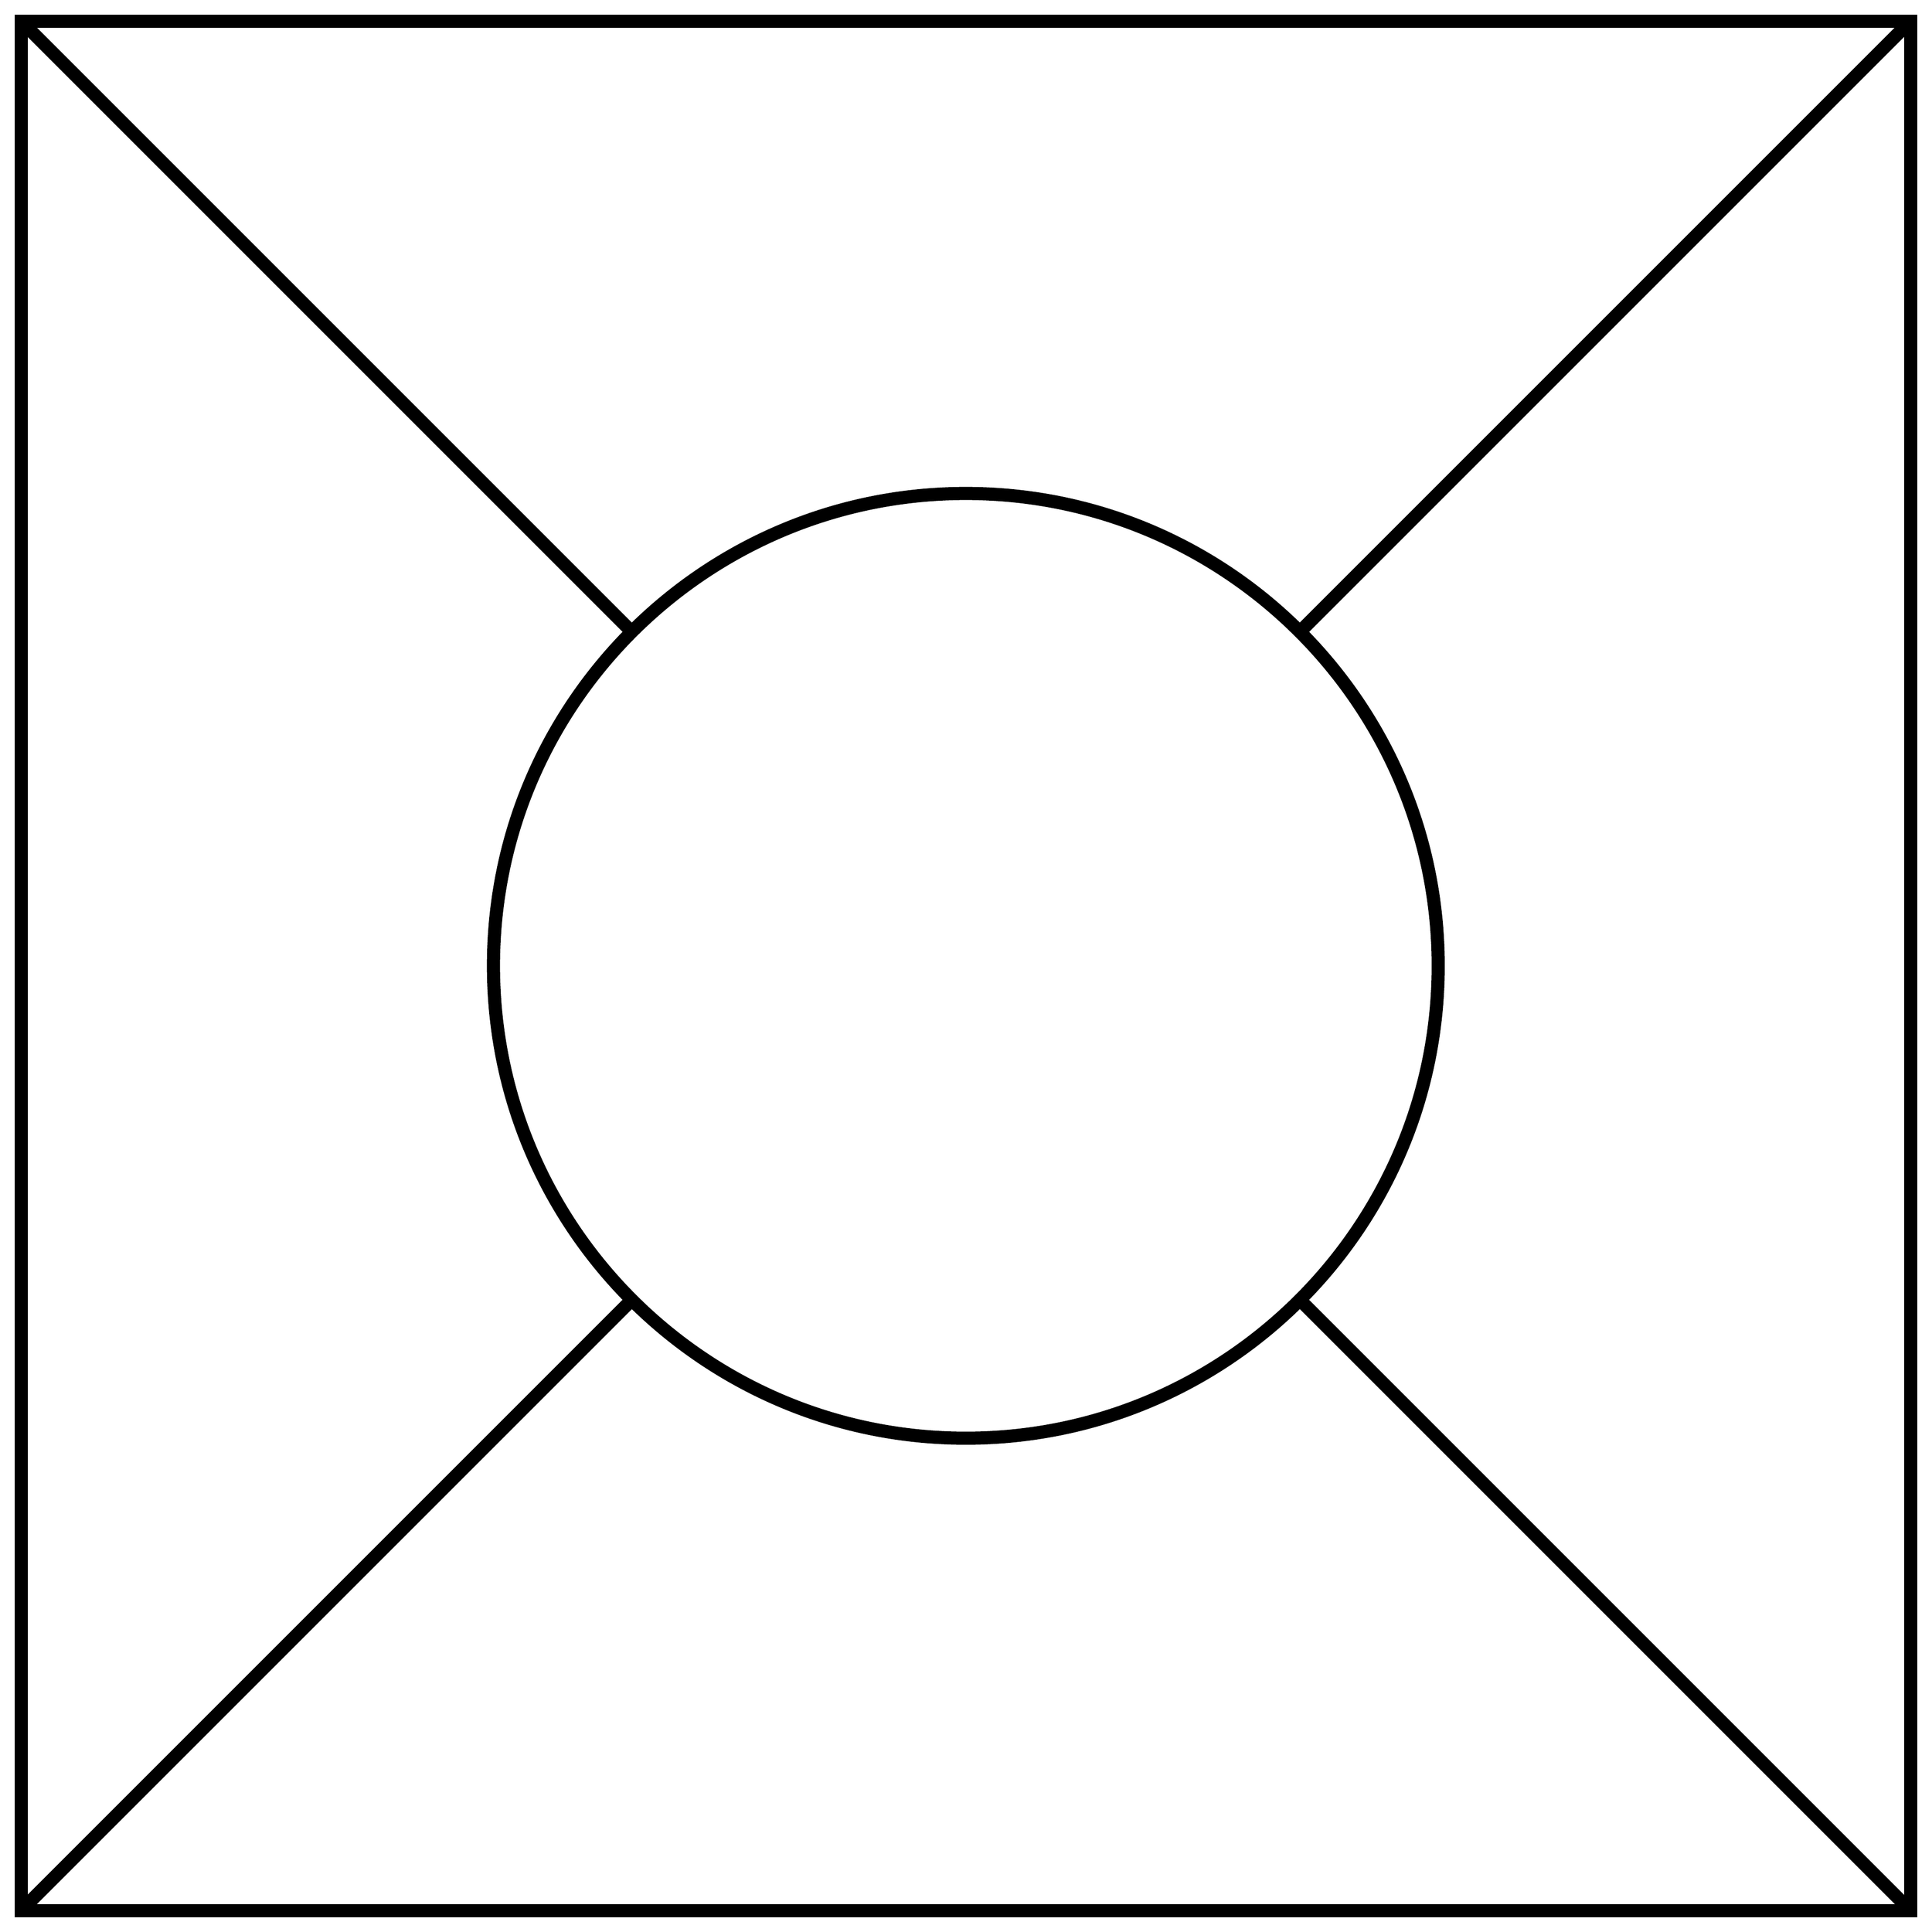
\begin{tikzpicture}
\draw[line width=0.125in] (-9in, -9in) rectangle (9in, 9in);
\draw[line width=0.125in] (-9in, -9in) -- (9in, 9in);
\draw[line width=0.125in] (-9in, 9in) -- (9in, -9in);
\node[draw, line width=0.125in, circle, fill=white, minimum size=9in, inner sep=0pt] at (0,0) {}; 
\end{tikzpicture}
\end{document}
